\documentclass[../DC2017114Bouma.tex]{subfiles}
\begin{document}
\graphicspath{{02_Material/img/}}
%% New chapter %%
\pagestyle{fancyreport}
\cleartooddpage
\pagestyle{fancyreport}
\chapter{Mechanical Systems with Unilateral Constraints and Spatial Friction}
In this chapter several modeling approaches of mechanical systems with unilateral constraints and spatial friction are presented. First a general representation of such a system is given, which is followed by sections introducing several formulations of the contact and friction laws in these systems. First a complementarity problem formulation is given, which is a complete and often used formulation for mechanical systems with unilateral constraints. From the complementarity formulation a hybrid system formulation is derived, which although less complete is a more intuitive formulation from a control point-of-view.
\section{General system definition}
\textbf{SOMEWHERE EXPLAIN DIFFERENCE BETWEEN CLOSING CONTACTS AND OTHER EVENTS (NONSMOOTHNESS)}\\
For mechanical systems a set of contact points $i_c\in\{i_1,i_2,...,i_C\}$ is defined, with $C$ being the number of considered contact points. A set $\Ic_\text{c}$ is defined as the set of closed contact points, such that a contact $i\in\Ic_\text{c}$ has closed a unilateral constraint. When a unilateral constraint is activated at a nonzero velocity impact happens, meaning a jump in the velocity will appear. Therefore the generalized velocity $\dot{\qb}$ is not continuously defined over the entire domain of a trajectory with impacts. Therefore $\xib:=\dot{\qb}$ is defined, except at impact-times $\tau_i$. Here $i$ is a counter for unilateral constraint activations where $i\in \{1,2,...,N\}$, with $N$ the amount of jumps in a trajectory. $h_n$ is the normal contact distance and $\zeta_{n,i_c}$ and $\zetab_{t,i_c}$ represent the relative velocities in normal and tangential direction,  respectively. 

\textbf{IMAGE HN ZETAN ZETAT}

Then, the continuous dynamics of a mechanical system with unilateral constraints and spatial friction are of the form
\begin{align}
&\Mb(\qb)\dot{\xib} + \Hb(\qb,\xib) = \Sb(\qb)\ub + \sum_{i_c\in\Ic_c}\left(\wb_{n,i_c}(\qb)\lambda_{n,i_c} + \Wb_{t,i_c}(\qb)\lambdab_{t,i_c} \right), \label{eq:appcont1}\\
&\text{(Contact Law)},\label{eq:appcont2}\\
&\text{(Friction Law)}.\label{eq:appcont3}
\end{align}
Here $\Mb(\qb)$ is the mass matrix of the system, $\Hb(\qb,\xib)$ contains the centripetal, Coriolis and gravitational forces in the system and $\Sb(\qb)$ represents the generalized directions of the forces. $\lambda_{n,i_c}$ and $\lambdab_{t,i_c}$ are the normal and tangential reaction forces, respectively, of contact point $i_c$ with $\wb_{n,i_c}$ and $\Wb_{t,i_c}$ the corresponding reaction force jacobians. When a contact point activates a unilateral constraint, impulsive dynamics can cause the state of the system to jump. These dynamics are of the form

\begin{align}
&\Mb(\qb)(\xib^+ - \xib^-) = \sum_{i_c\in\Ic_c}\left( \wb_{n,i_c}(\qb)\Lambda_{n,i_c} + \Wb_{t,i_c}(\qb)\Lambdab_{t,i_c}\right), \label{eq:appimp1}\\
&\text{(Impulsive Contact Law)},\label{eq:appimp2}\\
&\text{(Impulsive Friction Law)}.\label{eq:appimp3}
\end{align}
Here $\Lambda_{n,i_c}$ and $\Lambdab_{t,i_c}$ the normal and tangential impulsive reaction forces, respectively, of contact point $i_c$. These dynamics are impulsive, and happen at one instance in time. The $^-$ superscript indicates the ante-event state and the $^+$ superscript indicates the post-event state. In the following sections three different methods of describing the contact and friction laws are presented. First a complementarity problem formulation of mechanical systems with unilateral constraints is given, from which later a proximal point formulation and a hybrid system formulation are derived. For more information on modeling of multibody systems one can refer to \cite{Leine2008} and \cite{Wouw2016}.

\section{Complementarity problem formulation}\label{sec:comp}
\subsection{Signorini's contact law and Poisson's impact law}
To describe the normal contact between rigid bodies Signorini's contact law is used. Since the bodies are impenetrable and reaction forces caused by contact can not prevent the bodies from seperating, both the contact distance $h_{n,i_c}$ and $\lambda_{n,i_c}$ can not become negative. Two situations are possible

\begin{enumerate}
\item $h_{n,i_c}=0\ \wedge\ \lambda_{n,i_c} \geq 0$ (closed-contact)
\item $h_{n,i_c}>0\ \wedge\ \lambda_{n,i_c} = 0$ (open-contact)
\end{enumerate}

These situations are illustrated in Figure~\ref{fig:signorinicontact}, where it can be seen that the two situations are orthogonal. This behavior can be summarized in the complementarity condition

\begin{align}
0\leq h_{n,i_c}\ \bot\ \lambda_{n,i_c} \geq 0,\label{eq:signorini}
\end{align}

where the symbol $\bot$ is used to express the orthogonality between $h_{n,i_c}$ and $\lambda_{n,i_c}$. The complementarity condition in \eqref{eq:signorini} is called Signorini's contact law.
\begin{figure}[h]
\centering
\begin{subfigure}{0.3\textwidth}
\centering
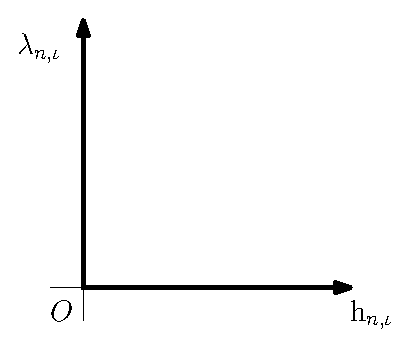
\includegraphics[width=\linewidth]{signorinicontact.eps}
\caption{Signorini's contact law.}\label{fig:signorinicontact}
\end{subfigure}
\qquad
%\begin{subfigure}{0.3\textwidth}
%\centering
%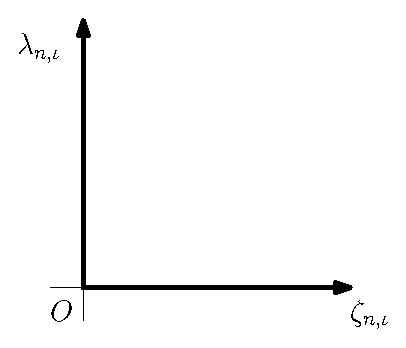
\includegraphics[width=\linewidth]{signoriniforce.eps}
%\caption{Signorini's force law.}\label{fig:signoriniforce}
%\end{subfigure}
%\quad
\begin{subfigure}{0.3\textwidth}
\centering
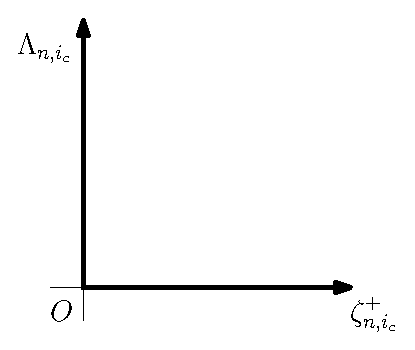
\includegraphics[width=\linewidth]{poissonimpact.eps}
\caption{Poisson's impact law without restitution.}\label{fig:poissonimpact}
\end{subfigure}
\caption{}
\end{figure}

When contact happens at nonzero velocity, impact occurs. Newton's impact law is used to describe this impact. Newton's law of impact is defined as
\begin{align}
\zeta^+_{n,i_c} = -e_{n,i_c}\zeta^-_{n,i_c},\text{ when }h_{n,i_c}=0,\ \dot{h}_{n,i_c}<0.
\end{align}
In this work the coefficient of restitution $e_{n,i_c}$ is assumed to be $0$, describing a completely inelastic contact. For closed contact an impact law can be defined that relates the impulsive contact force $\Lambda_{n,i_c}$ to the post-impact normal velocity $\zeta_{n,i_c}$. When considering multi-contact systems, when a contact is closed two situations can occur:
\begin{enumerate}
\item $\Lambda_{n,i_c} > 0\ \wedge\ \zeta^+_{n,i_c} = 0$ (impact)
\item $\Lambda_{n,i_c} = 0\ \wedge\ \zeta^+_{n,i_c} \geq 0$ (no impact)
\end{enumerate}
The second case can occur when a contact point other than $i_c$ makes impact. The situations described above are illustrated in Figure~\ref{fig:poissonimpact}, where again the orthogonality can be observed. The behavior is written into the complementarity condition

\begin{align}
0\leq \zeta^+_{n,i_c}\ \bot\ \Lambda_{n,i_c} \geq 0,\quad  \qquad \forall i_c\in\Ic_c,\label{eq:poisson}
\end{align}

with $\Ic_c$ the set of closed contacts. The complementarity condition \eqref{eq:poisson} is called Poisson's impact law. Note that the impact law is defined on velocity level, whereas the contact law is defined on position level.
\subsection{Coulomb's friction law}
Coulomb's friction law is often used to describe dry friction in mechanical systems. When considering 3-dimensional environments, Coulomb's friction law is defined as 

\begin{align}
||\lambdab_{t,i_c}||\ \in\ \left\{ \begin{array}{ll}
||\lambdab_{t,i_c}||\leq\mu\lambda_{n,i_c}, &\text{if }||\zetab_{t,i_c}||=0\\
||\lambdab_{t,i_c}|| = \mu\lambda_{n,i_c}, &\text{if }||\zetab_{t,i_c}||>0
\end{array}\right.,\label{eq:frictionlen}
\end{align}
and since friction is considered isotropic
\begin{align}
\zetab_{t,i_c} = -\kappa_{i_c}\frac{\lambdab_{t,i_c}}{||\lambdab_{t,i_c}||}.\label{eq:frictiondir}
\end{align}
with $\kappa_{i_c}>0$.

\eqref{eq:frictionlen} can be considered as a relation between the magnitude of the tangential velocity $\zetab_{t,i_c}$ and the reaction friction force $\lambdab_{t,i_c}$. \eqref{eq:frictiondir} can be considered as a relation between the direction of $\zetab_{t,i_c}$ and $\lambdab_{t,i_c}$, namely that $\zetab_{t,i_c}$ and $\lambdab_{t,i_c}$ are always in opposite directions. The constant $\kappa_{i_c}$ can then be interpreted as the magnitude of the tangential velocity. Coulomb's friction law is illustrated in Figure~\ref{fig:coulombfriction}. In Figure~\ref{fig:coulombort} the same law is illustrated, but now as orthogonal vectors. As noticed earlier, this is convenient for writing the law in a complementarity form.

\begin{figure}[h]
\centering
\begin{subfigure}{0.38\textwidth}
\centering
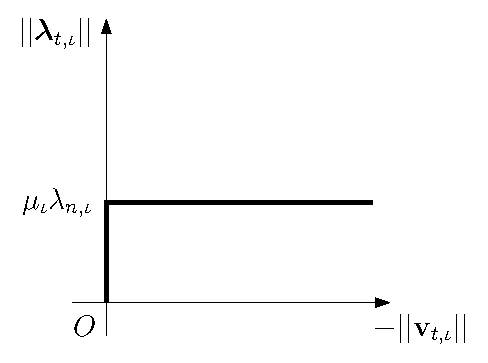
\includegraphics[width=\linewidth]{coulombfriction.eps}\caption{Coulomb's friction law.}\vspace{1.25cm}\label{fig:coulombfriction}
\end{subfigure}
\qquad
\begin{subfigure}{0.3\textwidth}
\centering
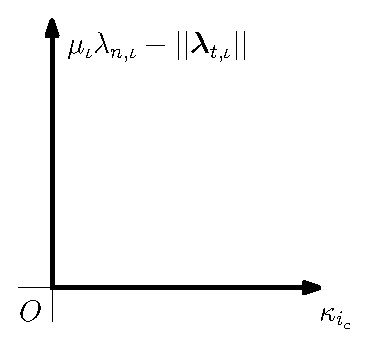
\includegraphics[width=\linewidth]{coulombort.eps}\caption{Coulomb's friction law as orthogonal vectors. $\kappa_{i_c}$ is defined as the magnitude of the tangential velocity $\zetab_{t,i_c}$.}\label{fig:coulombort}
\end{subfigure}
\end{figure}

The complementarity formulation of the Coulomb's law is therefore defined as

\begin{align}
&0\leq \left(\mu\lambda_{n,i_c} - ||\lambdab_{t,i_c}||\right)\ \bot\ \kappa_{i_c} \geq 0,\label{eq:coulomb1}\\
&||\lambdab_{t,i_c}||\zetab_{t,i_c} = -\kappa_{i_c}\lambdab_{t,i_c}.\label{eq:coulomb2}
\end{align}

\eqref{eq:frictiondir} is rewritten to \eqref{eq:coulomb2} to avoid singularity problems for $||\lambdab_{t,i_c}|| = 0$. For the impulsive behavior of the friction law Newton's impact law is used to define the tangential post-impact velocity as
\begin{align}
\zetab^+_{t,i_c} = -e_{t,i_c}\zetab^-_{t,i_c},
\end{align}
where in this work $e_{t,i_c}=0$ is assumed. Then, similarly to the non-impulsive case, the impulsive Coulomb's friction law can be defined as
\begin{align}
&0 \leq (\mu\Lambda_{n,i_c} - ||\Lambdab_{t,i_c}||)\ \bot\ \kappa_{i_c} \geq 0. \qquad \forall i_c\in\Ic_c,\label{eq:coulombimp1}\\
&||\Lambdab_{t,i}||\zetab_{t,i_c}^+ = \kappa_{i_c}\Lambdab_{t,i_c},\qquad \forall i_c\in\Ic_c.\label{eq:coulombimp2}
\end{align}
Note that just as the contact case, the impulsive friction law only holds for closed contacts.
\subsection{System dynamics with contact and friction law}
The flow dynamics are then described by
\begin{align}
&\Mb(\qb)\dot{\xib} + \Hb(\qb,\xib) = \Sb(\qb)\ub + \sum_{i\in\Ic_c}\left(\wb_{n,i}(\qb)\lambda_{n,i} + \Wb_{t,i}(\qb)\lambdab_{t,i} \right), \label{eq:ncpcontact1}\\
&0\leq h_{n,i}\ \bot\ \lambda_{n,i} \geq 0,\label{eq:ncpcontact2}\\
&0\leq \left(\mu\lambda_{n,i} - ||\lambdab_{t,i}||\right)\ \bot\ \kappa_i \geq 0,\label{eq:ncpcontact3}\\
&||\lambdab_{t,i}||\zetab_{t,i} = -\kappa_i\lambdab_{t,i},\label{eq:ncpcontact4}
\end{align}
with 
\begin{align}
&h_{n,i} = \wb_{n,i}^T(\qb)\qb,\label{eq:h}\\
&\zeta_{n,i}(\qb) = \wb^T_{n,i}(\qb) \xib,  \label{eq:zetan}\\
&\zetab_{t,i}(\qb) = \Wb^T_{t,i}(\qb) \xib. \label{eq:zetab}
\end{align}
The impulsive dynamics that take place when a contact point opens or closes contact are described by
\begin{align}
&\Mb(\qb)(\xib^+ - \xib^-) = \sum_{i\in\Ic_c}\left( \wb_{n,i}(\qb)\Lambda_{n,i} + \Wb_{t,i}(\qb)\Lambdab_{t,i}\right), \label{eq:ncpimpact1}\\
&0\leq \zeta_{n,i}^+\ \bot\ \Lambda_{n,i} \geq 0, \qquad \forall i\in\Ic_c,\label{eq:ncpimpact2}\\
&0 \leq (\mu\Lambda_{n,i} - ||\Lambdab_{t,i}||)\ \bot\ \kappa_i \geq 0. \qquad \forall i\in\Ic_c,\label{eq:ncpimpact3}\\
&||\Lambdab_{t,i}||\zetab_{t,i}^+ = -\kappa_i\Lambdab_{t,i},\qquad \forall i\in\Ic_c,\label{eq:ncpimpact4}
\end{align}
with 
\begin{align}
&\zeta^+_{n,i}(\qb) = \wb^T_{n,i}(\qb) \xib^+,\\
&\zetab^+_{t,i}(\qb) = \Wb^T_{t,i}(\qb) \xib^+.\label{eq:ncpimpactend}
\end{align}

\section{Hybrid system formulation}
In this section the dynamics of the complementarity system defined in Section~\ref{sec:comp} is written to a hybrid formulation, resulting in a hybrid framework for mechanical systems with unilateral constraints and spatial friction. The hybrid system formulation only holds for trajectories where only the contact points activating a guard function are allowed to change mode, i.e. no superfluous contacts. More information on the considered trajectories in this work is given in Section~\ref{app:trajectories}.

\subsection{Hybrid systems with impulsive effects}
According to \cite{Haddad2006} an impulsive dynamical system can be described by a hybrid system with impulsive effects. This makes it a valid framework for mechanical systems with unilateral constraints and spatial friction. The notation given in \cite{Haddad2006} is convenient from a tracking point-of-view, in that only the dynamics encountered during the trajectory need to be described. A hybrid system with impulsive effects consists of three elements:
\begin{enumerate}
\item Continuous dynamics, a continuous-time differential equation which defines the behavior of the system in between events
\item Discrete dynamics, which defines the way the state of the system is reset during events
\item Reset sets, which is a criterion to decide when the state of the system is to be reset
\end{enumerate}

Therefore, a hybrid system with impulsive effects is given by

\begin{equation}
\begin{array}{ll}
\dot{\xb}(t,i) =\ ^{s_i}\fb(\xb(t,i),\ub(t,i),t),& \xb(t,i),\ub(t,i)\notin \ ^{s_i}D\\
\xb(t,i) = \ ^{s_i}\gb(\xb(t,i-1),\ub(t,i-1),t),& \xb(t,i-1),\ub(t,i-1)\in \ ^{s_i}D
\end{array}\label{eq:hybimp}
\end{equation}
with $\xb(t,i)\in\Rbb^{n(s_i)}$, $\ub(t,i)\in\Rbb^{m(s_i)}$, $\ ^{s_i}\fb(t,i)\ :\ \Rbb^{n(s_i)}\ \times\ \Rbb^{m(s_i)}\ \times\ \Rbb\rightarrow \Rbb^{n(s_i)}$. $s_i$ is the mode descriptor of the system during flow after event $i$. Note that the state dimension $n(s_i)$ and the input dimension $m(s_i)$ can vary in different modes $s_i$. For the difference equation we have $\ ^{s_i}\gb\ :\ \Rbb^{n(s_{i-1})}\ \times\ \Rbb^{m(s_{i-1})}\ \times\ \Rbb\rightarrow \Rbb^{n(s_i)}$. The set $\ ^{s_i}D = \ ^{s_i}D(t) := \{\xb(t,i)\in\Rbb^{n(s_i)},\ \ub(t,i)\in\Rbb^{m(s_i)}\ |\ ^{s_i}_{=}\gamma(\xb^{\wedge},\ub^{\wedge},t) = 0, \ ^{s_i}_{\geq}\gamma(\xb^{\wedge},\ub^{\wedge},t) \geq 0\}$, where $\ ^{s_i}_{=}\gamma$ and $\ ^{s_i}_{\geq}\gamma$ are some sets of guard functions that are activated at event $i$, and $\xb^{\wedge}$,$\ub^{\wedge}$ are some virtual state and input that are not necessarily physically realistic.

The dynamics given in \eqref{eq:hybimp} will be used to describe a tracking problem for mechanical systems with unilateral constraints and spatial friction. A nominal state-input trajectory is considered consisting of absolutely continuous segments $(\alphab(t,i),\mub(t,i))$, with $t\in\left[\tau_i,\tau_{i+1}\right]$ and $i\in\{0,1,...,N\}$ the event counter. $\alphab(t,i)$ and $\mub(t,i)$ are the nominal state and input, respectively, that define the nominal trajectory with $N$ events. $\tau_i$ is referred to as the nominal event time of event $i$ and $t$ is referred to as regular time. Every segment of the nominal trajectory $(\alphab(t,i),\mub(t,i))$ and every event $i\in\{0,1,...,N\}$ satisfy the dynamics in \eqref{eq:hybimp}, where an event happens when $(\alphab(t,i),\mub(t,i))$ enters $\ ^{s_{i+1}}D$. Such a nominal trajectory existing of absolutely continuous segments experiencing events according to \eqref{eq:hybimp} is illustrated in Figure~\ref{fig:nomtraj}.

\begin{figure}[h]
\centering
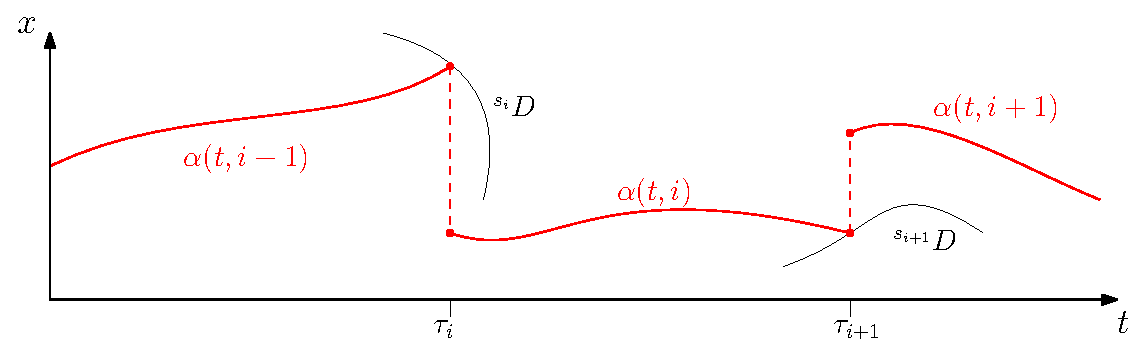
\includegraphics[width=\textwidth]{nomtraj.eps}\caption{A nominal trajectory consisting of two events and three segments, which satisfies the dynamics \eqref{eq:hybimp}. At the nominal event time $\tau_i$ the trajectory governed by $\dot{\alphab}(t,i-1) =\ ^{s_{i-1}}\fb(\alphab(t,i-1),\mub(t,i-1),t)$ enters the set $\ ^{s_i}D$, which leads to a state jump described by $\alphab(t,i) = \ ^{s_i}\gb(\alphab(t,i-1),\mub(t,i-1),\tau_i)$. After event $i$ the flow continues according to $\dot{\alphab}(t,i) =\ ^{s_i}\fb(\alphab(t,i),\mub(t,i),t)$. Note that the jump only happens in the state $\alphab$ and not in $\mub$.} \label{fig:nomtraj}
\end{figure}

The following sections will be used to write the complementarity system defined in Section~\ref{sec:comp} into a hybrid system with impulsive effects as in \eqref{eq:hybimp}. In \ref{sec:2contdyn} the continuous dynamics $\ ^{s_i}\fb$ will be derived for mechanical systems with unilateral constraints and spatial friction. Then, in Section~\ref{sec:2discdyn} the discrete dynamics $\ ^{s_i}\gb$ of the hybrid system with impulsive effects will be derived. Finally, in Section~\ref{sec:2reset} the reset set $\ ^{s_i}D$ will be defined. This will fully define the hybrid system with impulsive effects formulation of mechanical systems with unilateral constraints and spatial friction.

\textbf{EXAMPLE WITH BLOCK PUSHING TO SURFACE, EXPLAIN $s_i$ HERE}\\
\textbf{IMAGE WITH TRAJECTORY AND ILLUSTRATIONS OF BLOCK NEXT TO IT}

\subsection{Continuous dynamics}\label{sec:2contdyn}
When describing mechanical systems, we take 

\begin{align}
\xb = \begin{bmatrix}
\qb\\ \dot{\qb}
\end{bmatrix},\quad
\dot{\xb} = \begin{bmatrix}
\dot{\qb}\\ \ddot{\qb}
\end{bmatrix},
\end{align}

where $\qb$ and $\dot{\qb}$ are the joint positions, velocities and accelerations respectively. As described in Section~\ref{sec:comp}, for mechanical systems a set of contact points $i_c\in\{i_1,i_2,...,i_C\}$ is defined. Here $C$ is the number of considered contact points. A set $\Ic_\text{c}$ is defined as the set of closed contact points, such that a contact $i\in\Ic_\text{c}$ has closed a unilateral constraint. The set $\Ic_\text{c}$ is subdivided in two subsets $\Ic_{\text{sl}}$ and $\Ic_{\text{st}}$, where $\Ic_{\text{sl}}$ is the set of closed contact points in slip and $\Ic_{\text{st}}$ the set of closed contact points in stick. Here $\Ic_\text{c} =\Ic_{\text{sl}}\cup\Ic_{\text{st}}$ and $\Ic_{\text{sl}}\cup\Ic_{\text{st}}=\emptyset$. 

\textbf{IMAGE ILLUSTRATING SETS}

The equations of motion, given in \eqref{eq:appcont1}, can be rewritten to

\begin{align}
\ddot{\qb} = \Mb^{-1}(\qb)\left[ \Sb(\qb)\ub - \Hb(\qb,\dot{\qb}) + \sum_{i_c\in\Ic_c}\left(\wb_{n,i_c}(\qb)\lambda_{n,i_c} + \Wb_{t,i_c}(\qb)\lambdab_{t,i_c} \right)\right].\label{eq:qddot}
\end{align}
Note that since $\ ^{s_i}\fb$ is only defined on $\xb(t,i),\ub(t,i)\notin \ ^{s_i}D$, it is not necessary to use $\xib$ to define the equations of motion as done in \eqref{eq:appcont1}. Now $\ ^{s_i}\fb$ can be written as

\begin{align}
\dot{\xb}(t,i) =\begin{bmatrix}
\dot{\qb}\\ \Mb^{-1}(\qb)\left[ \Sb(\qb)\ub - \Hb(\qb,\dot{\qb}) + \sum_{i_c\in\Ic_c}\left(\wb_{n,i_c}(\qb)\lambda_{n,i_c} + \Wb_{t,i_c}(\qb)\lambdab_{t,i_c} \right)\right]
\end{bmatrix}.\label{eq:fcont}
\end{align}

The closed contact points in $\Ic_\text{c}$ experience reaction forces $\lambda_{n,i_c}$ and $\lambdab_{t,i_c}$, as can be seen in \eqref{eq:qddot}. Therefore for all closed contact points $i_c\in\Ic_\text{c}$ constraints are given which define these reaction forces. These constraints are given by

\begin{equation}
\begin{array}{ll}
\wb^T_{n,i}(\qb)\ddot{\qb} + \dot{\wb}^T_{n,i}(\qb)\dot{\qb} = 0, & \forall i_c\in\Ic_{\text{c}},\\
\Wb^T_{t,i}(\qb)\ddot{\qb} + \dot{\Wb}^T_{t,i}(\qb)\dot{\qb} = 0, & \forall i_c\in\Ic_{\text{sl}},\\
||\zetab^-_{t,i}||\lambdab_{t,i} + \zetab^-_{t,i}\mu\lambda_{n,i} = 0, & \forall i_c\in\Ic_{\text{st}},
\end{array}\label{eq:fcontconst}
\end{equation}
where $\Ic_{\text{sl}}$ and $\Ic_{\text{st}}$ are the sets of closed contacts in slip and closed contacts in stick respectively. Now, with \eqref{eq:fcont} and \eqref{eq:fcontconst}, the continuous dynamics of the hybrid system with impulsive dynamics are correctly defined.

\textbf{DO WE NEED APPENDIX WITH MORE THOROUGH DERIVATION?}

\subsection{Discrete dynamics}\label{sec:2discdyn}
\textbf{Define transition maps based on contact point sets}
The impact dynamics related to the jump sets are given by
\begin{align}
&0\leftarrow \ast:\nonumber\\
&(\dot{\qb}^+ - \dot{\qb}^-) = 0,\label{eq:appjump1}\\
&1\leftarrow\ast:\nonumber\\
&\Mb(\qb)(\dot{\qb}^+ - \dot{\qb}^-) = \wb_{n,i}(\qb)\Lambda_{n,i} + \Wb_{t,i}(\qb)\Lambdab_{t,i},\label{eq:appjump2}\\
&\zeta_{n,i}^+=0,\label{eq:appjump3}\\
&\Lambdab_{t,i} = -\widehat{\zetab}^-_{t,i}\mu\Lambda_{n,i},\label{eq:appjump4}\\
&2\leftarrow \ast:\nonumber\\
&\Mb(\qb)(\dot{\qb}^+ - \dot{\qb}^-) = \wb_{n,i}(\qb)\Lambda_{n,i} + \Wb_{t,i}(\qb)\Lambdab_{t,i},\label{eq:appjump5}\\
&\zeta_{n,i}^+=0,\label{eq:appjump6}\\
&\zeta_{t,i}^+= 0,\label{eq:appjump7}
\end{align}
with $0\leftarrow\ast$,$1\leftarrow\ast$ and $2\leftarrow\ast$ representing the impact dynamics to open contact, slip and stick respectively. 

When we go from any mode to open, there is no jump in the velocity and the reaction impulses are 0. Therefore $0\leftarrow \ast$ is correct.

When we go from open to slip, there will be a jump in velocity, and $||\Lambdab_{t,i}|| = \mu\Lambda_{n,i}$. The reaction impulses will be larger than zero. When we go from stick to slip, there will be no jump in velocity. In stick, $\zetab_{t,i} =0$, so $\epsilon(\zetab^-_{t,i}) = 0$. Also we know $\wb_{n,i}^T\dot{\qb}^- = \wb_{n,i}^T\dot{\qb}^+ = 0 $. This leads to $\dot{\qb}^- = \dot{\qb}^+$, meaning there is no jump in velocity and no impulsive reaction force. Therefore $1\leftarrow \ast$ is correct.

When we go from open to stick, there will be a jump in velocity and impulsive reaction forces.
\textbf{SHOW THAT JUMP MAPS ARE CORRECT}

\subsection{Reset sets}\label{sec:2reset}
\textbf{Open to stick/slip}\\
When a contact point is "open", it can trigger a guard function $\gamma$ to go from open to closed.

\textbf{DEFINITION OF $\gamma$}

The plane that spans $\gamma = 0$ is divided in two regions: a region where the post-impact state is in slip and a region where the post-impact state is in stick. This region is defined by $\Gamma$, where $\Gamma<0$ in the region where the contact point goes to slip and $\Gamma > 0$ in the region where the contact point goes to stick. When $\Gamma = 0$ the system is right at the border between a slip post-impact state and a stick post-impact state. This is illustrated in Figure~\ref{fig:guardopcl}. 

\begin{figure}[H]
	\centering
	\includegraphics[width=.7\textwidth]{guardopcl.eps}\caption{The functions $\gammab(\qb,\dot{\qb})$ and $\Gammab(\qb,\dot{\qb})$ illustrated in the state space of $\qb\in\mathbb{R}^{2}$. The light blue area is the state space where the contact is open, and goes the closed when it triggers $\gamma = 0$. If it triggers $\gamma = 0$ in the area where $\Gamma<0$ (orange), then the contact will go to slip. If it triggers $\gamma=0$ in the area where $\Gamma\geq 0$ (green), then the contact will go to stick.}\label{fig:guardopcl}
\end{figure}

For slip, we know that $\mu\Lambda_{n,i} - ||\Lambdab_{t,i}|| = 0$ and for stick, we know that  $\mu\Lambda_{n,i} - ||\Lambdab_{t,i}|| \geq 0$. From this we can derive the guard function
\begin{align}
\Gamma = \mu^2 \Lambda_{n,i}^2(\qb,\dot{\qb}^-) - \Lambdab_{t,i}(\qb,\dot{\qb}^-)\Lambdab_{t,i}^T(\qb,\dot{\qb}^-). \label{eq:slipset}
\end{align}
This guard function $\Gamma$ satisfies the requirements that $\Gamma<0$ in the region where the contact point goes to slip, $\Gamma > 0$ in the region where the contact point goes to stick and $\Gamma = 0$ at the border. Even though it is not physically realistic that $\Gamma < 0$, it can still be used as a guard-function.
We now find expressions for $\Lambda_{n,i}$ and $\Lambdab_{t,i}$ by looking at the jump map to stick, given in \eqref{eq:appjump5} to \eqref{eq:appjump7}.

We can rewrite \eqref{eq:appjump5} to
\begin{align}
\dot{\qb}^+ = \Mb^{-1}\wb_{n,i}\Lambda_{n,i} + \Mb^{-1}\Wb_{t,i}\Lambdab_{t,i} + \dot{\qb}^-,
\end{align}
which after substituting into \eqref{eq:appjump6} and \eqref{eq:appjump7} lead to

\begin{align}
\wb_{n,i}^T\Mb^{-1}\wb_{n,i}\Lambda_{n,i} + \wb_{n,i}^T\Mb^{-1}\Wb_{t,i}\Lambdab_{t,i} + \zeta_{n,i}^- = 0\\
\Wb_{t,i}^T\Mb^{-1}\wb_{n,i}\Lambda_{n,i} + \Wb_{t,i}^T\Mb^{-1}\Wb_{t,i}\Lambdab_{t,i} + \zetab_{t,i}^- = 0,
\end{align}
respectively, with $\zeta_{n,i}^- = \wb_{n,i}^T\dot{\qb}^-$ and $\zetab_{t,i}^- = \Wb_{t,i}^T\dot{\qb}^-$. This is now rewritten to

\begin{align}
\begin{bmatrix}
\wb_{n,i}^T\Mb^{-1}\wb_{n,i} & \wb_{n,i}^T\Mb^{-1}\Wb_{t,i} \\
\Wb_{t,i}^T\Mb^{-1}\wb_{n,i} & \Wb_{t,i}^T\Mb^{-1}\Wb_{t,i}
\end{bmatrix}
\begin{bmatrix}
\Lambda_{n,i}\\
\Lambdab_{t,i}
\end{bmatrix} + \begin{bmatrix}
\zeta_{n,i}^-\\
\zetab_{t,i}^-
\end{bmatrix}
= 0,
\end{align}
which is in turn rewritten to
\begin{align}
\begin{bmatrix}
\Lambda_{n,i}\\
\Lambdab_{t,i}
\end{bmatrix} = - \Db^{-1}\begin{bmatrix}
\zeta_{n,i}^-\\
\zetab_{t,i}^-
\end{bmatrix},\quad \text{with } \Db = \begin{bmatrix}
\wb_{n,i}^T\Mb^{-1}\wb_{n,i} & \wb_{n,i}^T\Mb^{-1}\Wb_{t,i} \\
\Wb_{t,i}^T\Mb^{-1}\wb_{n,i} & \Wb_{t,i}^T\Mb^{-1}\Wb_{t,i}
\end{bmatrix}.
\end{align}

The matrix $\Db$ is often called a Delassus-matrix. We now have expressions for $\Lambda_{n,i}$ and $\Lambdab_{t,i}$ which are continuous and differentiable in $(\qb,\dot{\qb})$. It is straightforward that $\Gamma(\qb,\dot{\qb})$ is continuous and differentiable as well.

\textbf{Stick to slip and slip to stick}\\

\textbf{Stick/slip to open}\\

\cleartooddpage
\chapter{Tracking Control for Hybrid Systems: Ordered State-Triggered Transitions}
\cite{Rijnen2017}\\
\textbf{Binary mode descriptor and $\eta$}\\
\textbf{Event character}\\

\section{Error notation for perturbed jump times}
\section{Linearization for Trajectories with Separate Guard-Activation}

\end{document}